% CVPR 2025 Paper Template; see https://github.com/cvpr-org/author-kit

\documentclass[10pt,twocolumn,letterpaper]{article}

%%%%%%%%% PAPER TYPE  - PLEASE UPDATE FOR FINAL VERSION
% \usepackage{cvpr}              % To produce the CAMERA-READY version
% \usepackage[review]{cvpr}      % To produce the REVIEW version
\usepackage[pagenumbers]{cvpr} % To force page numbers, e.g. for an arXiv version

% Import additional packages in the preamble file, before hyperref
%
% --- inline annotations
%
\newcommand{\red}[1]{{\color{red}#1}}
\newcommand{\todo}[1]{{\color{red}#1}}
\newcommand{\TODO}[1]{\textbf{\color{red}[TODO: #1]}}
% --- disable by uncommenting  
% \renewcommand{\TODO}[1]{}
% \renewcommand{\todo}[1]{#1}



% It is strongly recommended to use hyperref, especially for the review version.
% hyperref with option pagebackref eases the reviewers' job.
% Please disable hyperref *only* if you encounter grave issues, 
% e.g. with the file validation for the camera-ready version.
%
% If you comment hyperref and then uncomment it, you should delete *.aux before re-running LaTeX.
% (Or just hit 'q' on the first LaTeX run, let it finish, and you should be clear).
\definecolor{cvprblue}{rgb}{0.21,0.49,0.74}
\usepackage[pagebackref,breaklinks,colorlinks,allcolors=cvprblue]{hyperref}

%%%%%%%%% PAPER ID  - PLEASE UPDATE
\def\paperID{*****} % *** Enter the Paper ID here
\def\confName{CVPR}
\def\confYear{2025}

%%%%%%%%% TITLE - PLEASE UPDATE
\title{Enhancing Image Segmentation: A Comparative Study}

%%%%%%%%% AUTHORS - PLEASE UPDATE
% \author{Aaryan\\
% IITH\\
% {\tt\small co21btech11001@iith.ac.in}
% % For a paper whose authors are all at the same institution,
% % omit the following lines up until the closing ``}''.
% % Additional authors and addresses can be added with ``\and'',
% % just like the second author.
% % To save space, use either the email address or home page, not both
% \and
% Aayush Kumar\\
% IITH \\
% {\tt\small co21btech11002@iith.ac.in}
% \and
% Darpan Gaur\\
% IITH\\
% {\tt\small co21btech11004@iith.ac.in}
% \and 
% Varun Gupta\\
% IITH\\
% {\tt\small cs21btech11060@iith.ac.in}
% }

% 4 authors with same institution
\author{Aaryan,  \quad  Aayush Kumar, \quad  Darpan Gaur, \quad  Varun Gupta\\
Indian Institute of Technology Hyderabad\\
{\tt\small \{co21btech11001, co21btech11002, co21btech11004, cs21btech11060\}@iith.ac.in}
}

\begin{document}
\maketitle
\begin{abstract}
    Image segmentation is a crucial task in computer vision with significant applications in various fields such as autonomous driving, medical imaging, and object detection. Accurate segmentation allows for precise identification and localization of objects within an image, which is essential for tasks that require detailed scene understanding. In this project, we aim to compare the performance of different image segmentation models, including Convolutional Neural Networks (CNNs), Graph Convolutional Networks (GraphCNNs), and Transformers. Our goal is to evaluate their effectiveness and identify the strengths and weaknesses of each approach in the context of image segmentation. This literature survey was greatly inspired by \cite{9356353}.
\end{abstract}    
\section{Introduction}
\label{sec:intro}

Please follow the steps outlined below when submitting your manuscript to the IEEE Computer Society Press.
This style guide now has several important modifications (for example, you are no longer warned against the use of sticky tape to attach your artwork to the paper), so all authors should read this new version.

%-------------------------------------------------------------------------
\subsection{Language}

All manuscripts must be in English.

\subsection{Dual submission}

Please refer to the author guidelines on the \confName\ \confYear\ web page for a
discussion of the policy on dual submissions.

\subsection{Paper length}
Papers, excluding the references section, must be no longer than eight pages in length.
The references section will not be included in the page count, and there is no limit on the length of the references section.
For example, a paper of eight pages with two pages of references would have a total length of 10 pages.
{\bf There will be no extra page charges for \confName\ \confYear.}

Overlength papers will simply not be reviewed.
This includes papers where the margins and formatting are deemed to have been significantly altered from those laid down by this style guide.
Note that this \LaTeX\ guide already sets figure captions and references in a smaller font.
The reason such papers will not be reviewed is that there is no provision for supervised revisions of manuscripts.
The reviewing process cannot determine the suitability of the paper for presentation in eight pages if it is reviewed in eleven.

%-------------------------------------------------------------------------
\subsection{The ruler}
The \LaTeX\ style defines a printed ruler which should be present in the version submitted for review.
The ruler is provided in order that reviewers may comment on particular lines in the paper without circumlocution.
If you are preparing a document using a non-\LaTeX\ document preparation system, please arrange for an equivalent ruler to appear on the final output pages.
The presence or absence of the ruler should not change the appearance of any other content on the page.
The camera-ready copy should not contain a ruler.
(\LaTeX\ users may use options of \texttt{cvpr.sty} to switch between different versions.)

Reviewers:
note that the ruler measurements do not align well with lines in the paper --- this turns out to be very difficult to do well when the paper contains many figures and equations, and, when done, looks ugly.
Just use fractional references (\eg, this line is $087.5$), although in most cases one would expect that the approximate location will be adequate.


\subsection{Paper ID}
Make sure that the Paper ID from the submission system is visible in the version submitted for review (replacing the ``*****'' you see in this document).
If you are using the \LaTeX\ template, \textbf{make sure to update paper ID in the appropriate place in the tex file}.


\subsection{Mathematics}

Please number all of your sections and displayed equations as in these examples:
\begin{equation}
  E = m\cdot c^2
  \label{eq:important}
\end{equation}
and
\begin{equation}
  v = a\cdot t.
  \label{eq:also-important}
\end{equation}
It is important for readers to be able to refer to any particular equation.
Just because you did not refer to it in the text does not mean some future reader might not need to refer to it.
It is cumbersome to have to use circumlocutions like ``the equation second from the top of page 3 column 1''.
(Note that the ruler will not be present in the final copy, so is not an alternative to equation numbers).
All authors will benefit from reading Mermin's description of how to write mathematics:
\url{http://www.pamitc.org/documents/mermin.pdf}.

\subsection{Blind review}

Many authors misunderstand the concept of anonymizing for blind review.
Blind review does not mean that one must remove citations to one's own work---in fact it is often impossible to review a paper unless the previous citations are known and available.

Blind review means that you do not use the words ``my'' or ``our'' when citing previous work.
That is all.
(But see below for tech reports.)

Saying ``this builds on the work of Lucy Smith [1]'' does not say that you are Lucy Smith;
it says that you are building on her work.
If you are Smith and Jones, do not say ``as we show in [7]'', say ``as Smith and Jones show in [7]'' and at the end of the paper, include reference 7 as you would any other cited work.

An example of a bad paper just asking to be rejected:
\begin{quote}
\begin{center}
    An analysis of the frobnicatable foo filter.
\end{center}

   In this paper we present a performance analysis of our previous paper [1], and show it to be inferior to all previously known methods.
   Why the previous paper was accepted without this analysis is beyond me.

   [1] Removed for blind review
\end{quote}


An example of an acceptable paper:
\begin{quote}
\begin{center}
     An analysis of the frobnicatable foo filter.
\end{center}

   In this paper we present a performance analysis of the  paper of Smith \etal [1], and show it to be inferior to all previously known methods.
   Why the previous paper was accepted without this analysis is beyond me.

   [1] Smith, L and Jones, C. ``The frobnicatable foo filter, a fundamental contribution to human knowledge''. Nature 381(12), 1-213.
\end{quote}

If you are making a submission to another conference at the same time, which covers similar or overlapping material, you may need to refer to that submission in order to explain the differences, just as you would if you had previously published related work.
In such cases, include the anonymized parallel submission~\cite{Authors14} as supplemental material and cite it as
\begin{quote}
[1] Authors. ``The frobnicatable foo filter'', F\&G 2014 Submission ID 324, Supplied as supplemental material {\tt fg324.pdf}.
\end{quote}

Finally, you may feel you need to tell the reader that more details can be found elsewhere, and refer them to a technical report.
For conference submissions, the paper must stand on its own, and not {\em require} the reviewer to go to a tech report for further details.
Thus, you may say in the body of the paper ``further details may be found in~\cite{Authors14b}''.
Then submit the tech report as supplemental material.
Again, you may not assume the reviewers will read this material.

Sometimes your paper is about a problem which you tested using a tool that is widely known to be restricted to a single institution.
For example, let's say it's 1969, you have solved a key problem on the Apollo lander, and you believe that the 1970 audience would like to hear about your
solution.
The work is a development of your celebrated 1968 paper entitled ``Zero-g frobnication: How being the only people in the world with access to the Apollo lander source code makes us a wow at parties'', by Zeus \etal.

You can handle this paper like any other.
Do not write ``We show how to improve our previous work [Anonymous, 1968].
This time we tested the algorithm on a lunar lander [name of lander removed for blind review]''.
That would be silly, and would immediately identify the authors.
Instead write the following:
\begin{quotation}
\noindent
   We describe a system for zero-g frobnication.
   This system is new because it handles the following cases:
   A, B.  Previous systems [Zeus et al. 1968] did not  handle case B properly.
   Ours handles it by including a foo term in the bar integral.

   ...

   The proposed system was integrated with the Apollo lunar lander, and went all the way to the moon, don't you know.
   It displayed the following behaviours, which show how well we solved cases A and B: ...
\end{quotation}
As you can see, the above text follows standard scientific convention, reads better than the first version, and does not explicitly name you as the authors.
A reviewer might think it likely that the new paper was written by Zeus \etal, but cannot make any decision based on that guess.
He or she would have to be sure that no other authors could have been contracted to solve problem B.
\medskip

\noindent
FAQ\medskip\\
{\bf Q:} Are acknowledgements OK?\\
{\bf A:} No.  Leave them for the final copy.\medskip\\
{\bf Q:} How do I cite my results reported in open challenges?
{\bf A:} To conform with the double-blind review policy, you can report results of other challenge participants together with your results in your paper.
For your results, however, you should not identify yourself and should not mention your participation in the challenge.
Instead present your results referring to the method proposed in your paper and draw conclusions based on the experimental comparison to other results.\medskip\\

\begin{figure}[t]
  \centering
  \fbox{\rule{0pt}{2in} \rule{0.9\linewidth}{0pt}}
   %\includegraphics[width=0.8\linewidth]{egfigure.eps}

   \caption{Example of caption.
   It is set in Roman so that mathematics (always set in Roman: $B \sin A = A \sin B$) may be included without an ugly clash.}
   \label{fig:onecol}
\end{figure}

\subsection{Miscellaneous}

\noindent
Compare the following:\\
\begin{tabular}{ll}
 \verb'$conf_a$' &  $conf_a$ \\
 \verb'$\mathit{conf}_a$' & $\mathit{conf}_a$
\end{tabular}\\
See The \TeX book, p165.

The space after \eg, meaning ``for example'', should not be a sentence-ending space.
So \eg is correct, {\em e.g.} is not.
The provided \verb'\eg' macro takes care of this.

When citing a multi-author paper, you may save space by using ``et alia'', shortened to ``\etal'' (not ``{\em et.\ al.}'' as ``{\em et}'' is a complete word).
If you use the \verb'\etal' macro provided, then you need not worry about double periods when used at the end of a sentence as in Alpher \etal.
However, use it only when there are three or more authors.
Thus, the following is correct:
   ``Frobnication has been trendy lately.
   It was introduced by Alpher~\cite{Alpher02}, and subsequently developed by
   Alpher and Fotheringham-Smythe~\cite{Alpher03}, and Alpher \etal~\cite{Alpher04}.''

This is incorrect: ``... subsequently developed by Alpher \etal~\cite{Alpher03} ...'' because reference~\cite{Alpher03} has just two authors.

\begin{figure*}
  \centering
  \begin{subfigure}{0.68\linewidth}
    \fbox{\rule{0pt}{2in} \rule{.9\linewidth}{0pt}}
    \caption{An example of a subfigure.}
    \label{fig:short-a}
  \end{subfigure}
  \hfill
  \begin{subfigure}{0.28\linewidth}
    \fbox{\rule{0pt}{2in} \rule{.9\linewidth}{0pt}}
    \caption{Another example of a subfigure.}
    \label{fig:short-b}
  \end{subfigure}
  \caption{Example of a short caption, which should be centered.}
  \label{fig:short}
\end{figure*}

% \section{Formatting your paper}
\label{sec:formatting}

All text must be in a two-column format.
The total allowable size of the text area is $6\frac78$ inches (17.46 cm) wide by $8\frac78$ inches (22.54 cm) high.
Columns are to be $3\frac14$ inches (8.25 cm) wide, with a $\frac{5}{16}$ inch (0.8 cm) space between them.
The main title (on the first page) should begin 1 inch (2.54 cm) from the top edge of the page.
The second and following pages should begin 1 inch (2.54 cm) from the top edge.
On all pages, the bottom margin should be $1\frac{1}{8}$ inches (2.86 cm) from the bottom edge of the page for $8.5 \times 11$-inch paper;
for A4 paper, approximately $1\frac{5}{8}$ inches (4.13 cm) from the bottom edge of the
page.

%-------------------------------------------------------------------------
\subsection{Margins and page numbering}

All printed material, including text, illustrations, and charts, must be kept
within a print area $6\frac{7}{8}$ inches (17.46 cm) wide by $8\frac{7}{8}$ inches (22.54 cm)
high.
%
Page numbers should be in the footer, centered and $\frac{3}{4}$ inches from the bottom of the page.
The review version should have page numbers, yet the final version submitted as camera ready should not show any page numbers.
The \LaTeX\ template takes care of this when used properly.



%-------------------------------------------------------------------------
\subsection{Type style and fonts}

Wherever Times is specified, Times Roman may also be used.
If neither is available on your word processor, please use the font closest in
appearance to Times to which you have access.

MAIN TITLE.
Center the title $1\frac{3}{8}$ inches (3.49 cm) from the top edge of the first page.
The title should be in Times 14-point, boldface type.
Capitalize the first letter of nouns, pronouns, verbs, adjectives, and adverbs;
do not capitalize articles, coordinate conjunctions, or prepositions (unless the title begins with such a word).
Leave two blank lines after the title.

AUTHOR NAME(s) and AFFILIATION(s) are to be centered beneath the title
and printed in Times 12-point, non-boldface type.
This information is to be followed by two blank lines.

The ABSTRACT and MAIN TEXT are to be in a two-column format.

MAIN TEXT.
Type main text in 10-point Times, single-spaced.
Do NOT use double-spacing.
All paragraphs should be indented 1 pica (approx.~$\frac{1}{6}$ inch or 0.422 cm).
Make sure your text is fully justified---that is, flush left and flush right.
Please do not place any additional blank lines between paragraphs.

Figure and table captions should be 9-point Roman type as in \cref{fig:onecol,fig:short}.
Short captions should be centred.

\noindent Callouts should be 9-point Helvetica, non-boldface type.
Initially capitalize only the first word of section titles and first-, second-, and third-order headings.

FIRST-ORDER HEADINGS.
(For example, {\large \bf 1. Introduction}) should be Times 12-point boldface, initially capitalized, flush left, with one blank line before, and one blank line after.

SECOND-ORDER HEADINGS.
(For example, { \bf 1.1. Database elements}) should be Times 11-point boldface, initially capitalized, flush left, with one blank line before, and one after.
If you require a third-order heading (we discourage it), use 10-point Times, boldface, initially capitalized, flush left, preceded by one blank line, followed by a period and your text on the same line.

%-------------------------------------------------------------------------
\subsection{Footnotes}

Please use footnotes\footnote{This is what a footnote looks like.
It often distracts the reader from the main flow of the argument.} sparingly.
Indeed, try to avoid footnotes altogether and include necessary peripheral observations in the text (within parentheses, if you prefer, as in this sentence).
If you wish to use a footnote, place it at the bottom of the column on the page on which it is referenced.
Use Times 8-point type, single-spaced.


%-------------------------------------------------------------------------
\subsection{Cross-references}

For the benefit of author(s) and readers, please use the
{\small\begin{verbatim}
  \cref{...}
\end{verbatim}}  command for cross-referencing to figures, tables, equations, or sections.
This will automatically insert the appropriate label alongside the cross-reference as in this example:
\begin{quotation}
  To see how our method outperforms previous work, please see \cref{fig:onecol} and \cref{tab:example}.
  It is also possible to refer to multiple targets as once, \eg~to \cref{fig:onecol,fig:short-a}.
  You may also return to \cref{sec:formatting} or look at \cref{eq:also-important}.
\end{quotation}
If you do not wish to abbreviate the label, for example at the beginning of the sentence, you can use the
{\small\begin{verbatim}
  \Cref{...}
\end{verbatim}}
command. Here is an example:
\begin{quotation}
  \Cref{fig:onecol} is also quite important.
\end{quotation}

%-------------------------------------------------------------------------
\subsection{References}

List and number all bibliographical references in 9-point Times, single-spaced, at the end of your paper.
When referenced in the text, enclose the citation number in square brackets, for
example~\cite{Authors14}.
Where appropriate, include page numbers and the name(s) of editors of referenced books.
When you cite multiple papers at once, please make sure that you cite them in numerical order like this \cite{Alpher02,Alpher03,Alpher05,Authors14b,Authors14}.
If you use the template as advised, this will be taken care of automatically.

\begin{table}
  \centering
  \begin{tabular}{@{}lc@{}}
    \toprule
    Method & Frobnability \\
    \midrule
    Theirs & Frumpy \\
    Yours & Frobbly \\
    Ours & Makes one's heart Frob\\
    \bottomrule
  \end{tabular}
  \caption{Results.   Ours is better.}
  \label{tab:example}
\end{table}

%-------------------------------------------------------------------------
\subsection{Illustrations, graphs, and photographs}

All graphics should be centered.
In \LaTeX, avoid using the \texttt{center} environment for this purpose, as this adds potentially unwanted whitespace.
Instead use
{\small\begin{verbatim}
  \centering
\end{verbatim}}
at the beginning of your figure.
Please ensure that any point you wish to make is resolvable in a printed copy of the paper.
Resize fonts in figures to match the font in the body text, and choose line widths that render effectively in print.
Readers (and reviewers), even of an electronic copy, may choose to print your paper in order to read it.
You cannot insist that they do otherwise, and therefore must not assume that they can zoom in to see tiny details on a graphic.

When placing figures in \LaTeX, it's almost always best to use \verb+\includegraphics+, and to specify the figure width as a multiple of the line width as in the example below
{\small\begin{verbatim}
   \usepackage{graphicx} ...
   \includegraphics[width=0.8\linewidth]
                   {myfile.pdf}
\end{verbatim}
}


%-------------------------------------------------------------------------
\subsection{Color}

Please refer to the author guidelines on the \confName\ \confYear\ web page for a discussion of the use of color in your document.

If you use color in your plots, please keep in mind that a significant subset of reviewers and readers may have a color vision deficiency; red-green blindness is the most frequent kind.
Hence avoid relying only on color as the discriminative feature in plots (such as red \vs green lines), but add a second discriminative feature to ease disambiguation.
% \section{Final copy}

You must include your signed IEEE copyright release form when you submit your finished paper.
We MUST have this form before your paper can be published in the proceedings.

Please direct any questions to the production editor in charge of these proceedings at the IEEE Computer Society Press:
\url{https://www.computer.org/about/contact}.
\section{Problem Statement}
This project aims to conduct a comprehensive comparative analysis of CNN, Transformer, and GNN-based approaches for image segmentation. These models will be evaluated using the dataset mentioned in the dataset section.  By leveraging the strengths of these architectures, we seek to identify their respective advantages and shortcomings. In addition to evaluating these architectures, we will implement a series of experiments designed to improve segmentation outcomes. Also, use the above analysis to the ongoing Kaggle competition focused on segmenting vasculature in 3D scans of human kidneys \cite{kaggle_competition}.
\section{Related Work}
\subsection{Convolutional Neural Networks}

Convolutional Neural Networks (CNNs) have become a standard approach for image segmentation tasks. This section discusses three important CNN architectures for segmentation: FCN, UNet++ and DeepLabV3+, providing a mathematical overview based on the foundational principles and improvements proposed in their respective works.

\subsubsection{Fully Convolutional Networks (FCN)}

The Fully Convolutional Network (FCN) \cite{long2015fcn} was one of the pioneering architectures for dense predictions in semantic segmentation. Unlike traditional CNNs, FCNs replace fully connected layers with convolutional layers, enabling the model to predict a segmentation mask with spatial dimensions corresponding to the input image. The core idea is to use convolutional and pooling layers to produce feature maps at various scales, followed by a deconvolution (upsampling) layer to restore the original image resolution.

The output of an FCN can be expressed as:
\[
\hat{y} = f(W \ast X + b)
\]
where $W$ represents the learned convolutional weights, $X$ is the input image, $b$ is the bias term, and $f$ is the activation function. Using convolutional layers throughout ensures the model can handle inputs of arbitrary sizes, and the final upsampling layer reconstructs the pixel-wise segmentation map.

\subsubsection{UNet++}

UNet++ \cite{zhou2019unet++} improves upon the original U-Net architecture by introducing nested and dense skip connections between the encoder and decoder paths, bridging the semantic gap between feature maps at different scales. This refinement reduces the complexity of the decoder and improves the network's ability to capture fine-grained details, particularly in medical imaging tasks.

The main innovation in UNet++ is the re-designed skip connections:
\[
F_{i,j} = H_{i,j} \left( F_{i-1,j} + \sum_{k=0}^{j-1} H_{i,k} \right)
\]
where $F_{i,j}$ represents the feature map at the $i$-th depth and $j$-th layer, and $H_{i,j}$ denotes the convolutional operations. The nested architecture allows for the gradual refinement of feature maps at each level, making it more effective in learning from complex and hierarchical data.

\subsubsection{DeepLabV3+}

DeepLabV3+ \cite{chen2018deeplabv3+} builds on DeepLabV3 by integrating an encoder-decoder structure and employing atrous (dilated) convolutions to capture multi-scale context efficiently. Atrous convolution introduces the dilation rate, $r$, which controls the spacing between kernel elements. This allows the network to expand the receptive field without increasing the number of parameters.

The atrous convolution operation is defined as:
\[
y[i] = \sum_k x[i + r \cdot k] \cdot w[k]
\]
where $x$ is the input, $w$ represents the filter weights, and $r$ is the dilation rate. DeepLabV3+ also includes an Atrous Spatial Pyramid Pooling (ASPP) module that applies multiple atrous convolutions with different rates, allowing the model to capture information at multiple scales. The decoder then upsamples the feature maps to generate the final segmentation mask.

\subsection{Graph Neural Networks: Graph-FCN and CNN-G}

Deep learning has made significant advancements in semantic segmentation by classifying pixels in images. However, during high-level feature extraction, it often ignores the local spatial information, which is important for accurate segmentation. Graph-based models address this limitation by including the missing local context.

\subsubsection{Graph-FCN}

Graph-FCN combines graph convolutional networks (GCNs) with fully convolutional networks (FCNs) to capture local spatial relationships in images. Initially, a convolutional network converts the image grid data into a graph structure, transforming the semantic segmentation task into a graph node classification problem. The graph convolutional network is then applied to classify the nodes in this graph, effectively solving the segmentation challenge.

FCN-16s generates feature maps, and node annotations are initialized by combining upsampled feature vectors and node locations. Labels for nodes are obtained by pooling the raw label image during training. The process is shown in Figure~\ref{fig:graphfcn_node_init}.

\begin{figure}
    \centering
    % \fbox{\rule{0pt}{2in} \rule{0.9\linewidth}{0pt}}
    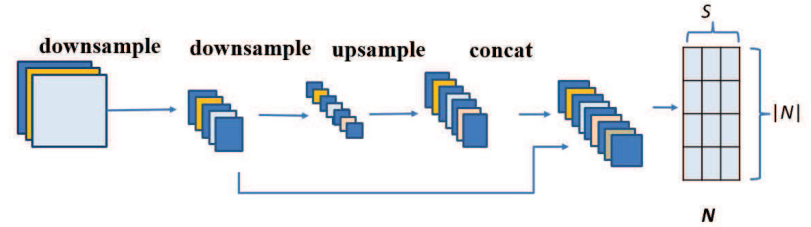
\includegraphics[width=0.8\linewidth]{images/graphfcn_node_init.png}
    \caption{Graph-FCN node initialization. From ~\cite{lu2020graphfcnimagesemanticsegmentation}.}
    \label{fig:graphfcn_node_init}
\end{figure}

In the graph model, edges are represented by an adjacency matrix, where each node is connected to its nearest $l$ nodes. These connections allow node annotations to transfer through the edges in the graph neural network.

FCN-16s handles node classification and graph model initialization on a small feature map, while a 2-layer GCN classifies the nodes within the graph. Cross-entropy loss is computed for both outputs, and like FCN-16s, Graph-FCN is trained end-to-end. The output of the prediction process is the output of the convolutional network. The graph model is only used during the training.

The structure of the Graph-FCN model is shown in Figure~\ref{fig:graphfcn_structure}.
\begin{figure}
    \centering
    % \fbox{\rule{0pt}{2in} \rule{0.9\linewidth}{0pt}}
    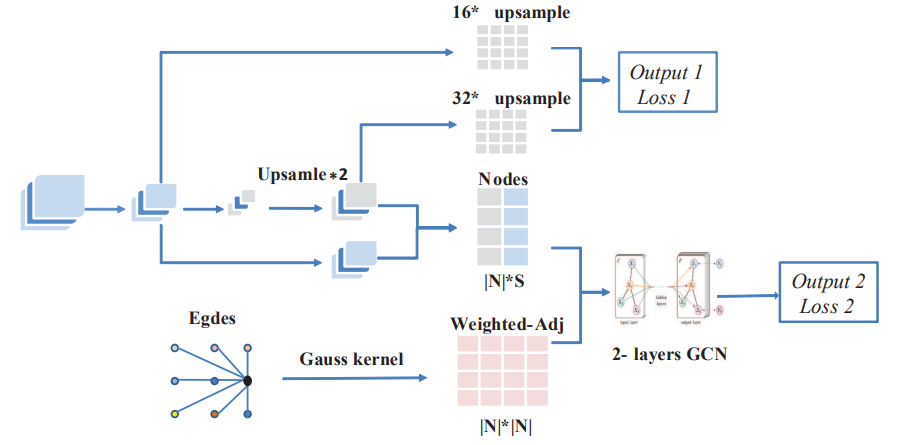
\includegraphics[width=0.8\linewidth]{images/graphfcn_structure.png}
    \caption{Graph-FCN model structure. From ~\cite{lu2020graphfcnimagesemanticsegmentation}.}
    \label{fig:graphfcn_structure}
\end{figure}

\subsubsection{CNN-G}

CNN-G builds on the Graph-FCN model by incorporating a graph-based approach with a convolutional neural network. Two types of structure models are used in CNN-G: distance-based and semantic-based, solved by GCN and GAT, respectively. The distance-based model captures the spatial relationships between nodes, while the semantic-based model focuses on the semantic relationships.

Using a graph attention network (GAT) enables flexible feature extraction across various receptive fields. This approach allows the model to integrate both structure learning and feature extraction.

\textbf{Distance-Based Structure:} Based on the assumption that the closer nodes are more correlated, the Gauss kernel function is used to generate the weighted edges.

The adjacent matrix $A = [e_{ij}]_{|N| \times |N|}$ is used to represent the edge set:

\[
e_{ij} = \begin{cases} \exp \left( -\frac{\|p_i - p_j\|^2}{\sigma^2} \right), & \text{an edge between } n_i \text{ and } n_j \\ 0, & \text{otherwise} \end{cases}.
\]

To simplify the calculation, we make the nodes connect to the $l$ closest nodes.

\textbf{Semantic-based model:} The initial attention coefficient $c_{ij}$ is used to measure the correlation between two nodes. The features of nodes with the same category will be more similar, the attention coefficient between each other will be larger, and the similarity is gradually strengthened in the iteration. A linear transformation is taken to map the concatenation of two nodes' features into a real number: 
\[
c_{ij} = a \left( n_i' || n_j' \right)
\]
The final attention coefficient is obtained through the normalization of all neighborhood nodes: 
\[
e_{ij} = \frac{\exp(c_{ij})}{\sum_{k \in neib_{i}} \exp(c_{ik})}.
\]
When the graph structure is unknown, the matrix $A_{\text{att}} = [e_{ij}]_{|N| \times |N|}$ can be taken as the adjacency matrix. In this case, the edge set is generated by the calculation of the attention coefficients.

In each case, the model generates two outputs, $y1$ and $y2$, which corresponds to two losses, $loss1$ and $loss2$. Both share the convolutional layer's extracted features. The final prediction is based on $y1$. Similar to Graph-FCN, the graph model is only used during training.

The structure of the CNN-G model is shown in Figure~\ref{fig:cnng_structure}.
\begin{figure}
    \centering
    % \fbox{\rule{0pt}{2in} \rule{0.9\linewidth}{0pt}}
    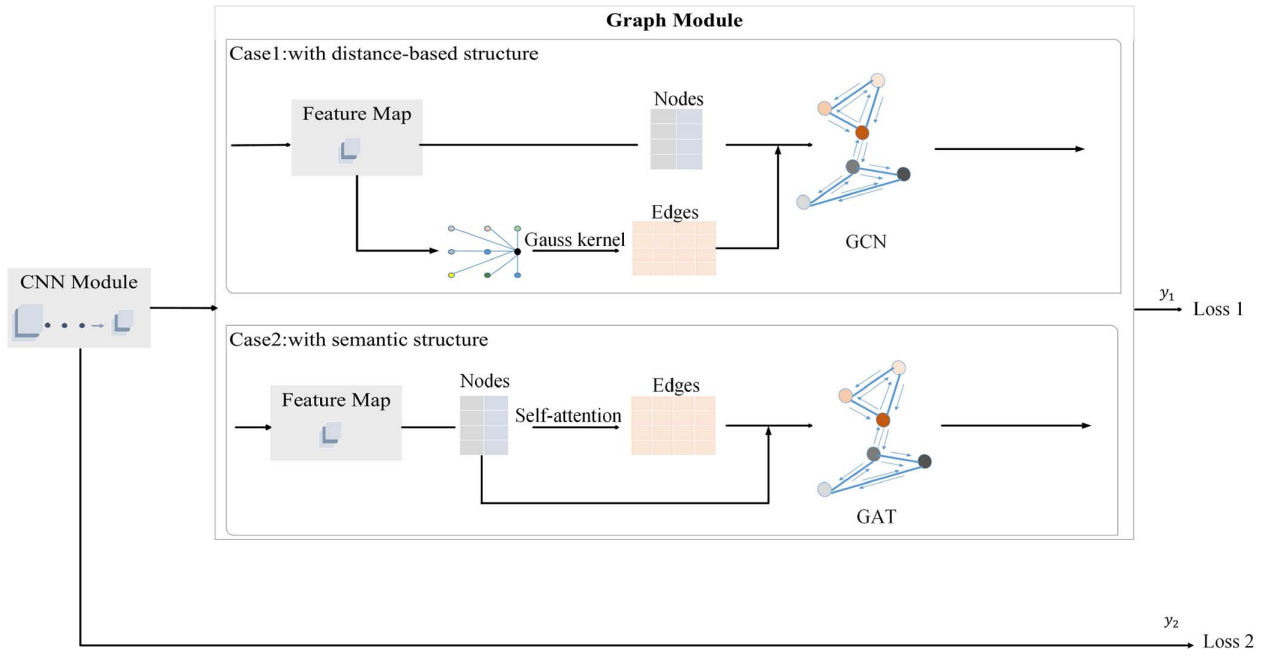
\includegraphics[width=0.8\linewidth]{images/cnng_structure.png}
    \caption{CNN-G model structure. From ~\cite{9103557}.}
    \label{fig:cnng_structure}
\end{figure}

\subsection{Transformer based approaches}
\subsubsection{TransUnet}
TransUNet \cite{chen2021transunettransformersmakestrong} has emerged as a robust framework for medical image segmentation by combining the strengths of U-Net and Transformer architectures.

TransUNet addresses these limitations by introducing a hybrid architecture that leverages both CNNs and Transformers. The encoder consists of a CNN followed by a Transformer module. The CNN is used to extract feature maps from the input images, which are then tokenized into image patches and fed into the Transformer. This CNN-Transformer hybrid allows TransUNet to capture detailed spatial features (via CNN) and global context (via the Transformer) simultaneously.

In the decoder, a cascaded upsampling module (CUP) is employed, consisting of multiple upsampling blocks with convolutional layers and ReLU activation. These upsampled features are combined with the high-resolution CNN feature maps from the encoder through skip connections, similar to the U-Net structure, enabling precise localization. This U-Net-like design ensures that TransUNet can recover lost spatial detail while preserving the high-level semantic understanding captured by the Transformer.

\subsubsection{Seg Former}
SegFormer \cite{xie2021segformersimpleefficientdesign} framework consists of two main modules: A hierarchical Transformer
encoder to extract coarse and fine features; and a lightweight All-MLP decoder to directly fuse these multi-level features and predict the semantic segmentation mask.
\begin{itemize}
    \item \textbf{Hierarchial Transformer Encoder}: designed to generate multi-scale features by progressively reducing the spatial resolution through a series of Mix Transformer (MiT) blocks. This encoder eliminates the need for positional encodings, making it adaptable to varying image sizes. Each MiT block employs overlapping patch embeddings and an efficient self-attention mechanism that reduces computational complexity, allowing it to handle high-resolution inputs. By producing features at multiple resolutions—{1/4, 1/8, 1/16, and 1/32} of the original size—it captures both local and global contexts for improved segmentation of complex objects. 
    \item \textbf{Lightweight All-MLP decoder}: It consists solely of MLP layers, which reduces computational overhead. The decoder first unifies the channel dimensions of the multi-level features, upsampling them to a common resolution before concatenation. This process enables the decoder to leverage fine-grained details and contextual information, ultimately generating a precise semantic segmentation mask. The lightweight design of the MLP decoder ensures high accuracy while maintaining low latency, making SegFormer suitable for real-time applications.
\end{itemize}

\subsubsection{Mask Former}
Mask Former \cite{cheng2021perpixelclassificationneedsemantic} architecture consists of three main components:
\begin{itemize}
    \item \textbf{Pixel-Level Module}: The pixel-level module extracts per-pixel embeddings from the image features. A backbone network (e.g., ResNet or Swin Transformer) first processes the input image to obtain low-resolution feature maps. These feature maps are then gradually upsampled using a lightweight pixel decoder based on the Feature Pyramid Network (FPN) to produce high-resolution, per-pixel embeddings.
    \item \textbf{Transformer Module}: The transformer module uses a standard decoder with learnable queries to compute global embeddings for each segment in the image. It takes the pixel-level features and processes them with multiple transformer decoder layers (6 by default). Each query represents a potential segment and generates a per-segment embedding, which encodes global information about the predicted mask.
    \item \textbf{Segmentation Module}: The segmentation module uses the segment embeddings from the transformer to produce a set of binary mask predictions and class labels. Each segment embedding is transformed into a mask embedding via a small Multi-Layer Perceptron (MLP). The mask embeddings are then combined with the per-pixel embeddings from the pixel-level module to generate binary masks using a dot-product operation. Finally, each binary mask is associated with a single global class prediction, and a classification loss is applied to these predictions. 
\end{itemize}


\section{Datasets}

There are a lot of 2D image datasets available for various purposes. Below is a list of some of the most popular:

\begin{itemize}
    \item \textbf{PASCAL Visual Object Classes (VOC)} is a dataset for object detection, segmentation, and classification. For the segmentation task, there are 21 labeled object classes and pixels are labeled as background if they do not belong to any of these classes. The dataset is divided into two sets, training and validation, with 1,464 and 1,449 images, respectively. An example image from the dataset is shown in Figure \ref{fig:pascal_voc}.
    \begin{figure}[t]
        \centering
         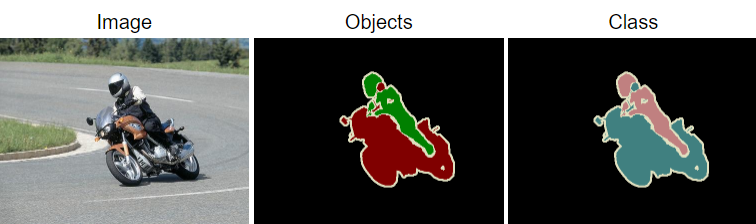
\includegraphics[width=0.8\linewidth]{images/pascal_voc.png}
      
         \caption{An example image from the PASCAL VOC dataset. From \cite{pascal_voc_dataset}}
         \label{fig:pascal_voc}
      \end{figure}
    \item \textbf{Cityscapes} contains a diverse set of stereo video sequences recorded in street scenes from 50 cities, with high-quality pixel-level annotation of 5,000 frames, in addition to a set of 20,000 weakly annotated frames. It includes semantic and dense pixel annotations of 30 classes, grouped into 8 categories — flat surfaces, humans, vehicles, constructions, objects, nature, sky, and void. An example image from the dataset is shown in Figure \ref{fig:cityscapes}.
    \begin{figure}[t]
        \centering
         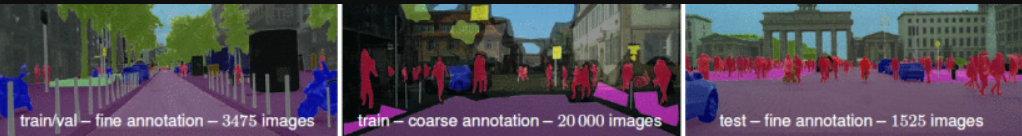
\includegraphics[width=0.8\linewidth]{images/cityscapes_example.png}
      
         \caption{An example image from the Cityscapes dataset. From \cite{7780719}}
         \label{fig:cityscapes}
      \end{figure}
\end{itemize}
\section{Evaluation Metrics}
\subsection{Pixel Accuracy}
Pixel accuracy is the ratio of correctly classified pixels divided by the total number of pixels. For $K+1$ classes ($K$ foreground classes and the background) pixel accuracy is defined as 
\begin{equation*} 
\text{PA}= \frac{\sum _{i=0}^K p_{ii}}{\sum _{i=0}^K \sum _{j=0}^K p_{ij}} 
\end{equation*} 
where $p_{ij}$ is the number of pixels of class $i$ predicted as belonging to class $j$.

\subsection{IoU Score}
Intersection over Union (IoU) is defined as the ratio of the area of intersection between the predicted segmentation map A and the ground truth map B to the area of their union.
\begin{equation*} 
\text{IoU}=  \frac{|A \cap B|}{|A \cup B|}. 
\end{equation*} 

\subsection{Dice Score}
Dice score is defined as twice the area of overlap between the predicted (map A) and ground-truth maps (map B), divided by the total number of pixels in both maps.
\begin{equation*} 
\text{Dice}= \frac{ 2| A \cap B |}{|A| + |B|}. 
\end{equation*} 
{
    \small
    \bibliographystyle{ieeenat_fullname}
    \bibliography{main}
}

% WARNING: do not forget to delete the supplementary pages from your submission 
% \clearpage
\setcounter{page}{1}
\maketitlesupplementary


\section{Rationale}
\label{sec:rationale}
% 
Having the supplementary compiled together with the main paper means that:
% 
\begin{itemize}
\item The supplementary can back-reference sections of the main paper, for example, we can refer to \cref{sec:intro};
\item The main paper can forward reference sub-sections within the supplementary explicitly (e.g. referring to a particular experiment); 
\item When submitted to arXiv, the supplementary will already included at the end of the paper.
\end{itemize}
% 
To split the supplementary pages from the main paper, you can use \href{https://support.apple.com/en-ca/guide/preview/prvw11793/mac#:~:text=Delete%20a%20page%20from%20a,or%20choose%20Edit%20%3E%20Delete).}{Preview (on macOS)}, \href{https://www.adobe.com/acrobat/how-to/delete-pages-from-pdf.html#:~:text=Choose%20%E2%80%9CTools%E2%80%9D%20%3E%20%E2%80%9COrganize,or%20pages%20from%20the%20file.}{Adobe Acrobat} (on all OSs), as well as \href{https://superuser.com/questions/517986/is-it-possible-to-delete-some-pages-of-a-pdf-document}{command line tools}.

\end{document}
